\subsection{La evolución de SOA: Microservicios}
\label{microservicios}

Como vimos en el apartado anterior, \gls{acro:soa} define qué principios debe cumplir un sistema distribuido para satisfacer los objetivos de la organización, que incluyen, facilidad y flexibilidad en la integración de sistemas \eng{legacy}, reducción en los costos de implementación y ágil adaptación a los cambios. Si bien esto ya establece precondiciones para un diseño, \gls{acro:soa} en sí no es un patrón concreto. Por el contrario, y similarmente a otros diseños de arquitectura de sistemas distribuidos como REST (el cual será tratado en la \autoref{standard:rest}), \gls{acro:soa} es un conjunto de propiedades que dichos sistemas debieran cumplir y a partir de los cuales podemos observar características comunes entre aquellos que sigan ese tipo de arquitecturas.

Es sobre la base de características de un tipo de sistemas como \gls{acro:soa} que se construyen luego los patrones de diseño. A modo de referencia se puede consultar el libro \eng{``SOA Patterns''} donde se definen más de 20 patrones orientados a servicios, como \eng{Service Host}\cite[p.~19]{soapatterns}, \eng{Composite Front End (Portal)}\cite[p.~148]{soapatterns} o \eng{Service Bus}\cite[p.162]{soapatterns}. Todos estos (y otros) patrones obedecen a los principios de las Arquitecturas Orientadas a Servicios, pero ninguno \textit{es} \gls{acro:soa} en sí mismo, ni \gls{acro:soa} \textit{es} solo uno de estos patrones. De hecho, si analizamos el caso particular de estos patrones podemos observar que inclusive pueden combinarse entre sí: el primero (\eng{Service Host}) guía en cómo se puede manejar el ambiente en que corren los servicios y los clientes de los mismos para simplificar su gestión, el segundo (\eng{Portal}) habla de cómo proveer una interfaz que combine más de un servicio, y el tercero (\eng{Service Bus}) propone la inclusión de un canal de comunicación previo a los servicios para gestionar las peticiones y respuestas con mejoras sobre la autogestión de peticiones por parte de los propios servicios.

En este contexto es que queremos centrarnos en un patrón de diseño de sistemas distribuidos emergente que se plantea como una alternativa al desarrollo de aplicaciones monolíticas.  Quizás el concepto mas importante para entender el patrón de arquitectura de microservicios, es el \eng{service component}.  En lugar de pensar en servicios para esta arquitectura, es mejor pensar en \eng{service components}, que pueden variar su granularidad, desde un simple módulo a gran parte de la aplicación.

Las aplicaciones monolíticas típicamente consisten en componentes fuertemente acoplados, que son parte de una única unidad desplegable (\eng{deployable}), resultando poco práctica y dificultosa la incorporación de cambios, \eng{testing} y \eng{deployment} de la aplicación. Es por esto que las grandes organizaciones de IT con aplicaciones de estas características, suelen manejarse con ciclos \textit{mensuales} de \eng{deployment} para sus productos.

El patrón de microservicios trata estas cuestiones, separando la aplicación en múltiples unidades \eng{deployables} (\eng{service components}), que pueden ser desarrolladas, testeadas y deployadas independientemente de otros \eng{service components}.\cite[p.~27]{richards2015}

Como puede observerse en \autoref{fig:basic_microservices_arquitecture_pattern}, las solicitudes de los clientes son realizadas a través de una capa denominada \eng{user interface layer}, para acceder finalmente a los \eng{service components}.

\begin{figure}[H]
  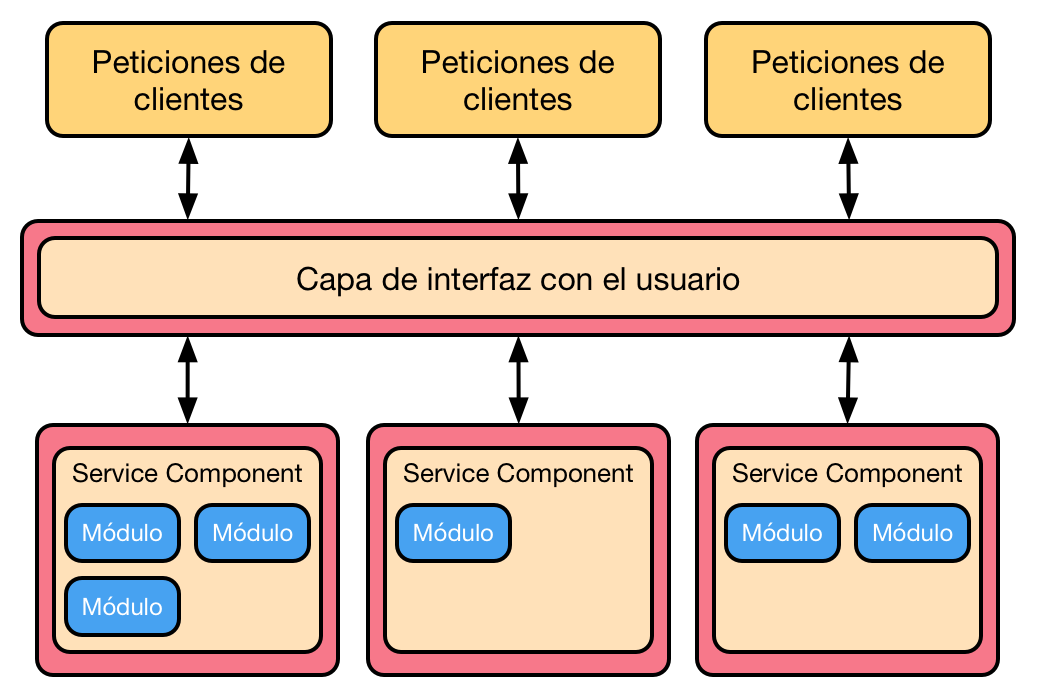
\includegraphics[width=\linewidth]{src/images/02-capitulo-2/basic_microservices_arquitecture_pattern.png}
  \caption{Arquitectura básica de microservicios}
  \label{fig:basic_microservices_arquitecture_pattern}
\end{figure}

Debido a que los componentes principales de una aplicación se dividen en partes mas pequeñas y deployables de manera individual, las aplicaciones construídas utilizando el patrón de arquitectura de microservicios son generalmente mas robustas, proporcionan una mejor escalabilidad y pueden dar soporte a una entrega contínuca (\eng{continuous delivery}), permitiendo actualizar los ambientes de producción mediante \eng{deployments} en tiempo real y \textit{en caliente}, reemplazando la necesidad de deployments mensuales o semanales. \cite[p.~33]{richards2015} Todo esto es posible, dado que el cambio generalmente se encuentra aislado a un \eng{service component}, y solo las unidades que cambian tienen que ser deployadas. Como se mencionó anteriormente, esta es una notable mejora frente al desarrollo de aplicaciones monolíticas, donde el fuerte acoplamiento en sus componentes deriva en aplicaciones \textit{frágiles} que suelen fallar con cada nuevo \eng{deployment} realizado.

Si bien existen decenas de formas para implementar el patrón de arquitectura de microservicios, las tres principales topologías son: \eng{API REST-based}, \eng{application REST-based}, y \eng{centralized messaging}.

Según lo investigado, entendemos que será necesario implementar la topología \eng{centralized messaging}\autoref{fig:centralized_messaging_topology}, la cual se adecúa a nuestra necesidades.  Esta topología es similar a la topología \eng{application REST-based}, solo que en lugar de utilizar REST para acceder remotamente a un \eng{service component}, utiliza un \eng{message broker} centralizado y liviano.  No hay que confundir esta topología con el patrón \gls{acro:soa} o consideralo como un ``SOA-Lite''.  Este \eng{message broker} no realiza orquestración, tranformación ni ruteo complejo, más bien, es sólo una capa de transporte ligera, para acceder a los \eng{services componets} remotos.  Los beneficios obtenidos con esta topología, en lugar de utilizar una topología sencilla \eng{REST-based} son: mecanismos avanzados de colas, mensajería asíncrona, monitoreo, control de errores, \eng{rate-limit}, seguridad, balanceo de carga y escalabilidad.

\begin{figure}[H]
  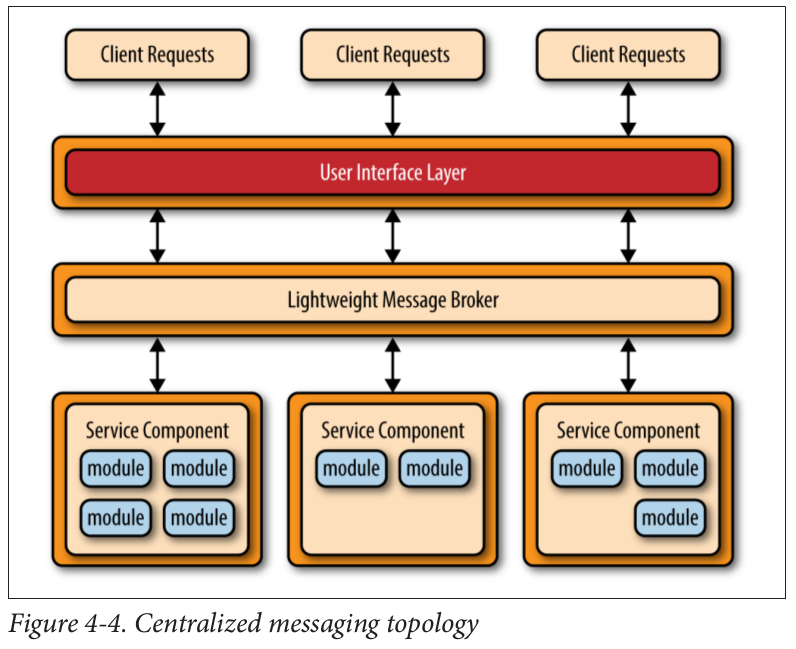
\includegraphics[width=\linewidth]{src/images/02-capitulo-2/centralized_messaging_topology.png}
  \caption{Centralized Messaging Topology}
  \label{fig:centralized_messaging_topology}
\end{figure}

El punto único de falla y el cuello de botella que se observa en esta arquitectura, puede ser abordado implementando un cluster de brokers, dividiendo una instancia del broker en múltiples instancias y repartiendo la carga en cada una de estas).\cite[p.~31]{richards2015}

Como se puede observar en \cite[p.~34]{richards2015}, se realiza un análisis de las siguientes características para el patrón de arquitectura de microservicios:

\begin{itemize}
  \item \textbf{Respuesta al cambio:} el autor indica que este patrón, tiene un alto grado de \eng{overall agility}, que es la habilidad de responder rápidamente a los constantes cambios en el entorno.  Dado que es posible deployar unidades de forma separada, los cambios se encuentran aislados a \eng{service components} individuales, lo que permite \eng{deployments} sencillos y rápidos.\\
  Además, aplicaciones desarrolladas con este patrón, tienden a generarse con bajo acoplamiento, lo que ayuda en la incorporación de los cambios.

  \item \textbf{\eng{Testability}:} dada la separación y aislamiento de las funcionalidad de negocio, las pruebas de regresión para un \eng{service component} en particular, resultan más sencillas y factibles que las mismas pruebas realizadas a toda una aplicación monolítica.  Además, ya que los \eng{service components} en este patrón están débilmente acoplados, hay menos posibilidades de que un desarrollador ``rompa'' la aplicación completa debido a la incorporación de un cambio reciente.

  \item \textbf{Rendimiento:} en general este patrón no aporta en el desarrollo de aplicaciones de alto rendimiento, debido a la naturaleza distribuida de la arquitectura de microservicios y el overhead que inherentemente agregan esas comunicaciones entre las unidades distribuidas.

  \item \textbf{Escalabilidad:} las aplicaciones se encuentran separadas en unidades deployables donde cada \eng{service component} puede escalarse individualmente, permitiendo afinar la escalabilidad de acuerdo a las necesidades de la aplicación lo cual resulta en una gran versatilidad para escalar partes de o un sistema completo.

  \item \textbf{Facilidad de desarrollo:} como la funcionalidad se encuentra separada en diferentes \eng{service components}, el desarrollo se vuelve mas sencillo debido a un alcance mas pequeño y asilado de cada unidad.
\end{itemize}
